%!Tex Root = ../Tutorat3.tex
% ./Packete.tex
% ./Design.tex
% ./Deklarationen.tex
% ./Aufgabe1.tex
% ./Aufgabe2.tex
% ./Aufgabe3.tex
% ./Aufgabe4.tex
% ./Bonus.tex

\section{Task 5}

\setcounter{task}{1}

\begin{frame}[allowframebreaks]{Task 5}{Earliest Deadline First – Star\vspace{0.5cm}}
  \begin{tasknoinc}
    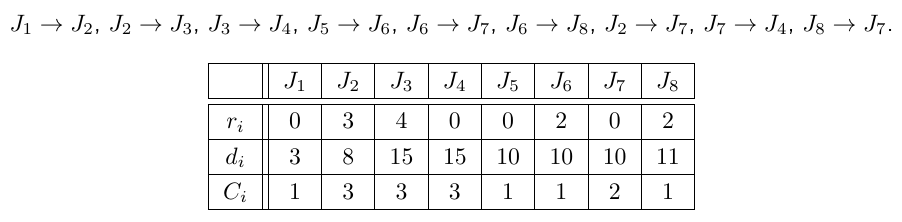
\includegraphics[width=\textwidth]{./figures/5_task.png}
    \begin{itemize}
      \item construct \alert{precedence graph}
    \end{itemize}
  \end{tasknoinc}
  \begin{solution}
    \centering
    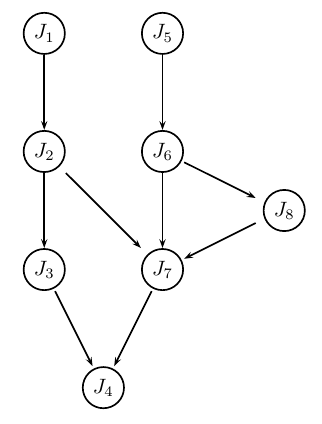
\includegraphics[width=0.3\textwidth]{./figures/5_graph.png}
  \end{solution}
\end{frame}

\begin{frame}[allowframebreaks]{Task 5}{Earliest Deadline First - Star\vspace{0.5cm}}
  \begin{tasknoinc}
    \begin{itemize}
      \item apply \alert{EDF* algorithm}
    \end{itemize}
    \centering
    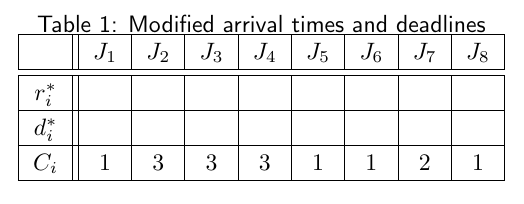
\includegraphics[width=0.5\textwidth]{./figures/5_table.png}
  \end{tasknoinc}
  \begin{solution}
    \centering
    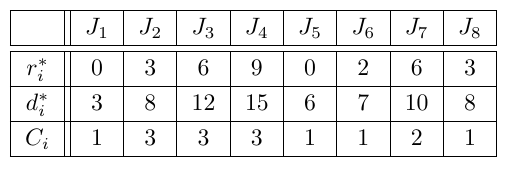
\includegraphics[width=0.5\textwidth]{./figures/5_table_sol.png}
  \end{solution}
\end{frame}

\begin{frame}[allowframebreaks]{Task 5}{Earliest Deadline First - Start\vspace{0.5cm}}
  \begin{tasknoinc}
    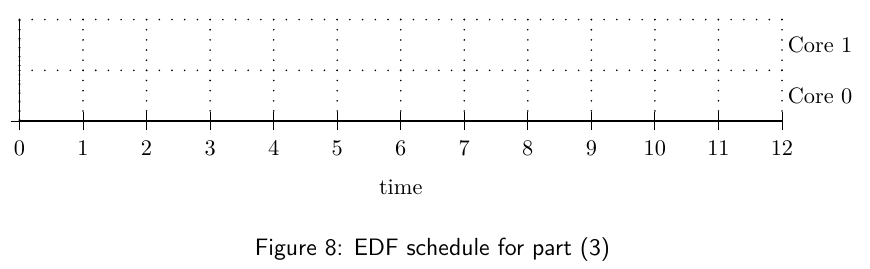
\includegraphics[width=\textwidth]{./figures/5_diag.png}
  \end{tasknoinc}
  \begin{solution}
    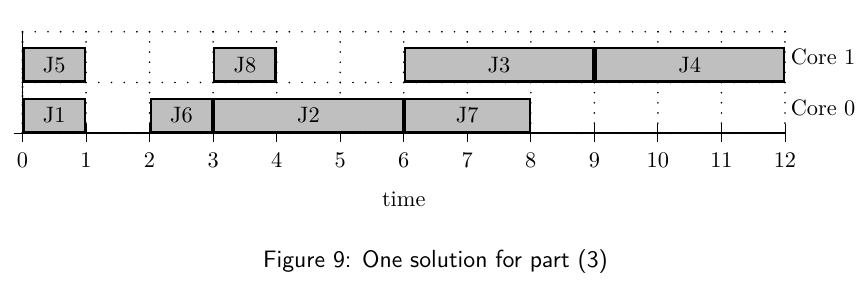
\includegraphics[width=\textwidth]{./figures/5_diag_sol.png}
  \end{solution}
\end{frame}

\begin{frame}[allowframebreaks]{Task 5}{Earliest Deadline First - Start\vspace{0.5cm}}
  \begin{tasknoinc}
    \begin{itemize}
      \item Will executing on the \alert{quad-core platform} with the same scheduling rule reduce the completion time of the application?
        \begin{itemize}
          \item $4$ cores execute the four ready tasks with earliest deadlines
        \end{itemize}
    \end{itemize}
  \end{tasknoinc}
  \begin{solution}
    \begin{itemize}
      \item No, $J_4$ cannot be started earlier than time $9$. Therefore, the minimum finish time of the application is $12$ (the finish time for the dual core platform)
    \end{itemize}
  \end{solution}
\end{frame}
